\begin{surferIntroPage}{Tutorial}{tutorial_koord1}{Aan de slag met SURFER}
Dit programma heet SURFER. Als je dit woord leest, denk je waarschijnlijk aan water, zon en golven. De naam komt hier echter van het Engelse woord {\it surface}, wat {\it oppervlak} betekent.
\\
Met SURFER kan je (algebra\"ische) oppervlakken visualiseren. Wat dit betekent en wat algebra\"ische oppervlakken juist zijn, wordt uitgelegd in deze tutorial. Kies \'e\'en van de oppervlakken rechts om door de verschillende hoofdstukken van de tutorial te bladeren.\\
SURFER is een deel van de rondtrekkende tentoonstelling IMAGINARY, die werd opgericht in het Duitse ``Jaar van de Wiskunde'' 2008. De tentoonstelling is een project van het internationaal bekende Mathematisches Forschungsinstitut Oberwolfach, dat in het Zwarte Woud gelegen is. Daar worden wekelijks workshops over actuele wiskundige thema's georganiseerd, waar wiskundigen van over de hele wereld kennis kunnen uitwisselen. \\
\vspace{0.2cm} \hspace{3.5cm}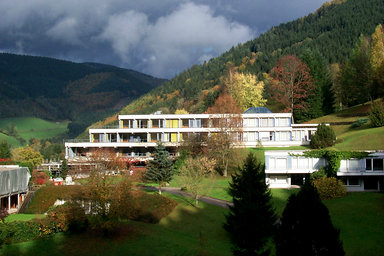
\includegraphics[width=3cm]{./../../common/images/photo_mfo.jpg}\\
Het SURFER programma kan je gratis downloaden op onze homepage: \\
\begin{centering}
www.imaginary.org\\
\end{centering}
 \vspace{0.2cm}
Aan de rechterkant kan je \'e\'en van de wiskundige tutorials kiezen, beginnend met het Citrus-oppervlak. Links kan je naar andere galerijen gaan, bijvoorbeeld naar de fantasie-oppervlakken.
\end{surferIntroPage}
